 \documentclass[xcolor=svgnames]{beamer}
%\documentclass[xcolor=svgnames, handout]{beamer}
%\includeonlyframes{current}


\usepackage[utf8]    {inputenc}
\usepackage[T1]      {fontenc}
\usepackage[english] {babel}

\usepackage{amsmath,amsfonts,graphicx}
\usepackage{beamerleanprogress}
\usepackage{xcolor}
\usepackage{soul}
%\usepackage{verbatim}
\usepackage{multicol}
\usepackage{tikz} 
\usepackage[export]{adjustbox}
\usepackage{fancyvrb}

\definecolor{iyellow}{RGB}{255, 162, 23}
\definecolor{sgreen}{RGB}{118, 191, 138}

\newcommand{\yellow}[1]{\textcolor{iyellow}{#1}}
\newcommand{\green}[1]{\textcolor{ForestGreen}{#1}}
\newcommand{\red}[1]{\textcolor{red}{#1}}
\newcommand{\blue}[1]{{\textcolor{blue}{#1}}}
\newcommand{\orange}[1]{{\textcolor{orange}{#1}}}
\newcommand{\bblue}[1]{\textcolor{SteelBlue!90!gray}{#1}} % beamer blue
\newcommand{\eol}{\\[1em]\pause}
\newcommand{\nl}{\\[1em]}
\newcommand{\define}[1]{\textbf{\textcolor{orange}{#1}}}
\newcommand{\answer}[1]{\textit{\textbf{\textcolor{iyellow}{#1}}}}
\newcommand{\command}[1]{\texttt{\textbf{\textcolor{DarkMagenta}{#1}}}}
\newcommand{\ipic}[2]{\includegraphics[width={#2}\textwidth]{#1}}

\usepackage{upquote}

%\newcommand{\newpt}{\par \vspace{5mm}}

\newcommand{\cell}[1]{{\sf \textbf{\textcolor{DarkMagenta}{#1}}}}
\newcommand{\ra}{$\rightarrow$}

\newcommand{\purple}[1]{{\textcolor{DarkMagenta}{#1}}}


\usepackage[T1]{fontenc}
\usepackage[utf8]{inputenc}
\usepackage{tikz}
\usetikzlibrary{shadows}
\hypersetup{colorlinks=true,linkcolor=blue, linktocpage}

\newcommand*\keystroke[1]{%
  \tikz[baseline=(key.base)]
    \node[%
      draw,
      fill=white,
      drop shadow={shadow xshift=0.25ex,shadow yshift=-0.25ex,fill=black,opacity=0.75},
      rectangle,
      rounded corners=2pt,
      inner sep=1pt,
      line width=0.5pt,
      font=\scriptsize\sffamily
    ](key) {#1\strut}
  ;
}

\usepackage{upquote}

\newcounter{myenumi}
\setcounter{myenumi}{0}
\newenvironment{myenumerate}{
\begin{enumerate}[{Exercise} \thelecture .1] 
\setcounter{enumi}{\value{myenumi}}
}{
\setcounter{myenumi}{\value{enumi}}
\end{enumerate}
}

% To create the above inline text (i.e. not with a list... acts like a new section would)
% found here: https://latex.org/forum/viewtopic.php?t=10815
\newcounter{exercise} \setcounter{exercise}{0}
 \renewcommand{\theexercise}{\arabic{lecture}.\arabic{exercise}}
\newenvironment{exercise}[1]%
{
\refstepcounter{exercise}
%\vspace{1ex}
%\flushleft\makebox[10ex][l]{\textbf{Ex} \thequestion} \texttt{#1}\\
%\flushleft\makebox[13ex][r]{\textbf{\bblue{Exercise}} \bblue{\thequestion}} {#1}\\
\flushleft{\textbf{\bblue{Exercise}} \bblue{\theexercise}} {#1}\\
}%
{}

\newcounter{subexercise}[exercise] \setcounter{subexercise}{0}
\renewcommand{\thesubexercise}{\arabic{lecture}.\arabic{exercise}.{\arabic{subexercise}}}
\newenvironment{subexercise}[1]%
{
\refstepcounter{subexercise}
\quad{\bblue{\thesubexercise}} {#1}\\
}%
{}




\usepackage{etoolbox}
\setbeamertemplate{theorems}[numbered]
\undef{\lemma}
\undef{\example}
\newtheorem{lemma}{\translate{Lemma}}
\theoremstyle{example}
\newtheorem{example}{\translate{Example}}
%\newcounter{question}[lecture]
%\newenvironment{question}[1][]{\refstepcounter{question}\par\medskip
%   \textbf{\green{Question~\thequestion. #1}} \rmfamily}{\medskip}


\renewcommand\thetheorem{\arabic{lecture}.\arabic{theorem}}
\renewcommand\theexample{\arabic{lecture}.\arabic{example}}
%\renewcommand\thequestion{\arabic{lecture}.\arabic{question}}
\makeatletter
\@addtoreset{theorem}{lecture}
\@addtoreset{example}{lecture}
%\@addtoreset{question}{lecture}
\makeatother


\newcommand{\ft}[1]{\frametitle{#1}}

\definecolor{mygreen}{cmyk}{0.82,0.11,1,0.25}
\newcommand{\ex}[1]{\textit{\textcolor{mygreen}{#1}}}
%\setbeamercovered{highly dynamic}
\newcounter{saveenumi}
\newcommand{\seti}{\setcounter{saveenumi}{\value{enumi}}}
\newcommand{\conti}{\setcounter{enumi}{\value{saveenumi}}}

\newenvironment{example*}
  {\addtocounter{example}{-1}\example}
  {\endexample}



\newtheorem{axiom}{Axiom}


\title
  [Data 301 Data Analytics\hspace{2em}]
  {Data 301 Data Analytics\\
Database Part II: SQL}

\author
  [Dr.\ Irene Vrbik]
  {Dr.\ Irene Vrbik}

\date
  {}

\institute
  {University of British Columbia Okanagan \newline irene.vrbik@ubc.ca}


\graphicspath{{img/}}

\begin{document}

\maketitle

\setbeamersize{description width=0.57cm} % to have less indent with the description environment

\setcounter{lecture}{5}
\section
  {SQL}


\begin{frame}{Intro}
\begin{itemize}
\item So far we've learnt how to manipulate data stored in a relational database using:
\begin{quote}
\begin{description}
\item[\command{CREATE}] to create new tables
\item[\command{INSERT}] to insert new rows
\item[\command{UPDATE}] to edit rows in a table 
\item[\command{ALTER}] to edit columns in a table 
\item[\command{DELETE}] for deleting rows
\item[\command{DROP TABLE}] for deleting tables
\end{description}
\end{quote}
\item Today we'll look at some examples for \emph{querying} data from a database.
\end{itemize}

\end{frame}


\begin{frame}{SQL Queries using \command{SELECT}}
A query in SQL has the form:
\begin{quote}
\begin{description}
          \item [\command{SELECT}]  {\tt <list of columns separated by commas>}
          \item [\command{FROM}]         {\tt      <list of tables>}
          \item [\command{WHERE}]      {\tt       <filter conditions>}
          \item [\command{GROUP BY}]   {\tt          <columns>}
          \item [\command{ORDER BY}]     {\tt       <columns>  ASC/DESC}
\end{description}
\end{quote}


Notes:
\begin{enumerate}
\item Separate the list of columns/expressions and list of tables by commas.
\item The "*" is used to select all columns.
\item Only \command{SELECT} required. \command{FROM, WHERE, GROUP BY, ORDER BY} are optional.
\end{enumerate}
\end{frame}


\frame{
\ft{Doing a query in SQL mode}
\begin{itemize}
\item To see how to do a basic \command{SELECT} query in Microsoft Access, see 1:35-2:25 in \href{https://www.youtube.com/watch?v=IFr4jvt_ZZc}{this} YouTube video.
\item To see how to do a basic \command{SELECT} query in LibreOffice base, see  \href{https://youtu.be/zG1IeZ37aj0}{this} YouTube demo.
\end{itemize}

}

\begin{frame}{Example Data}
\vspace{-3em}
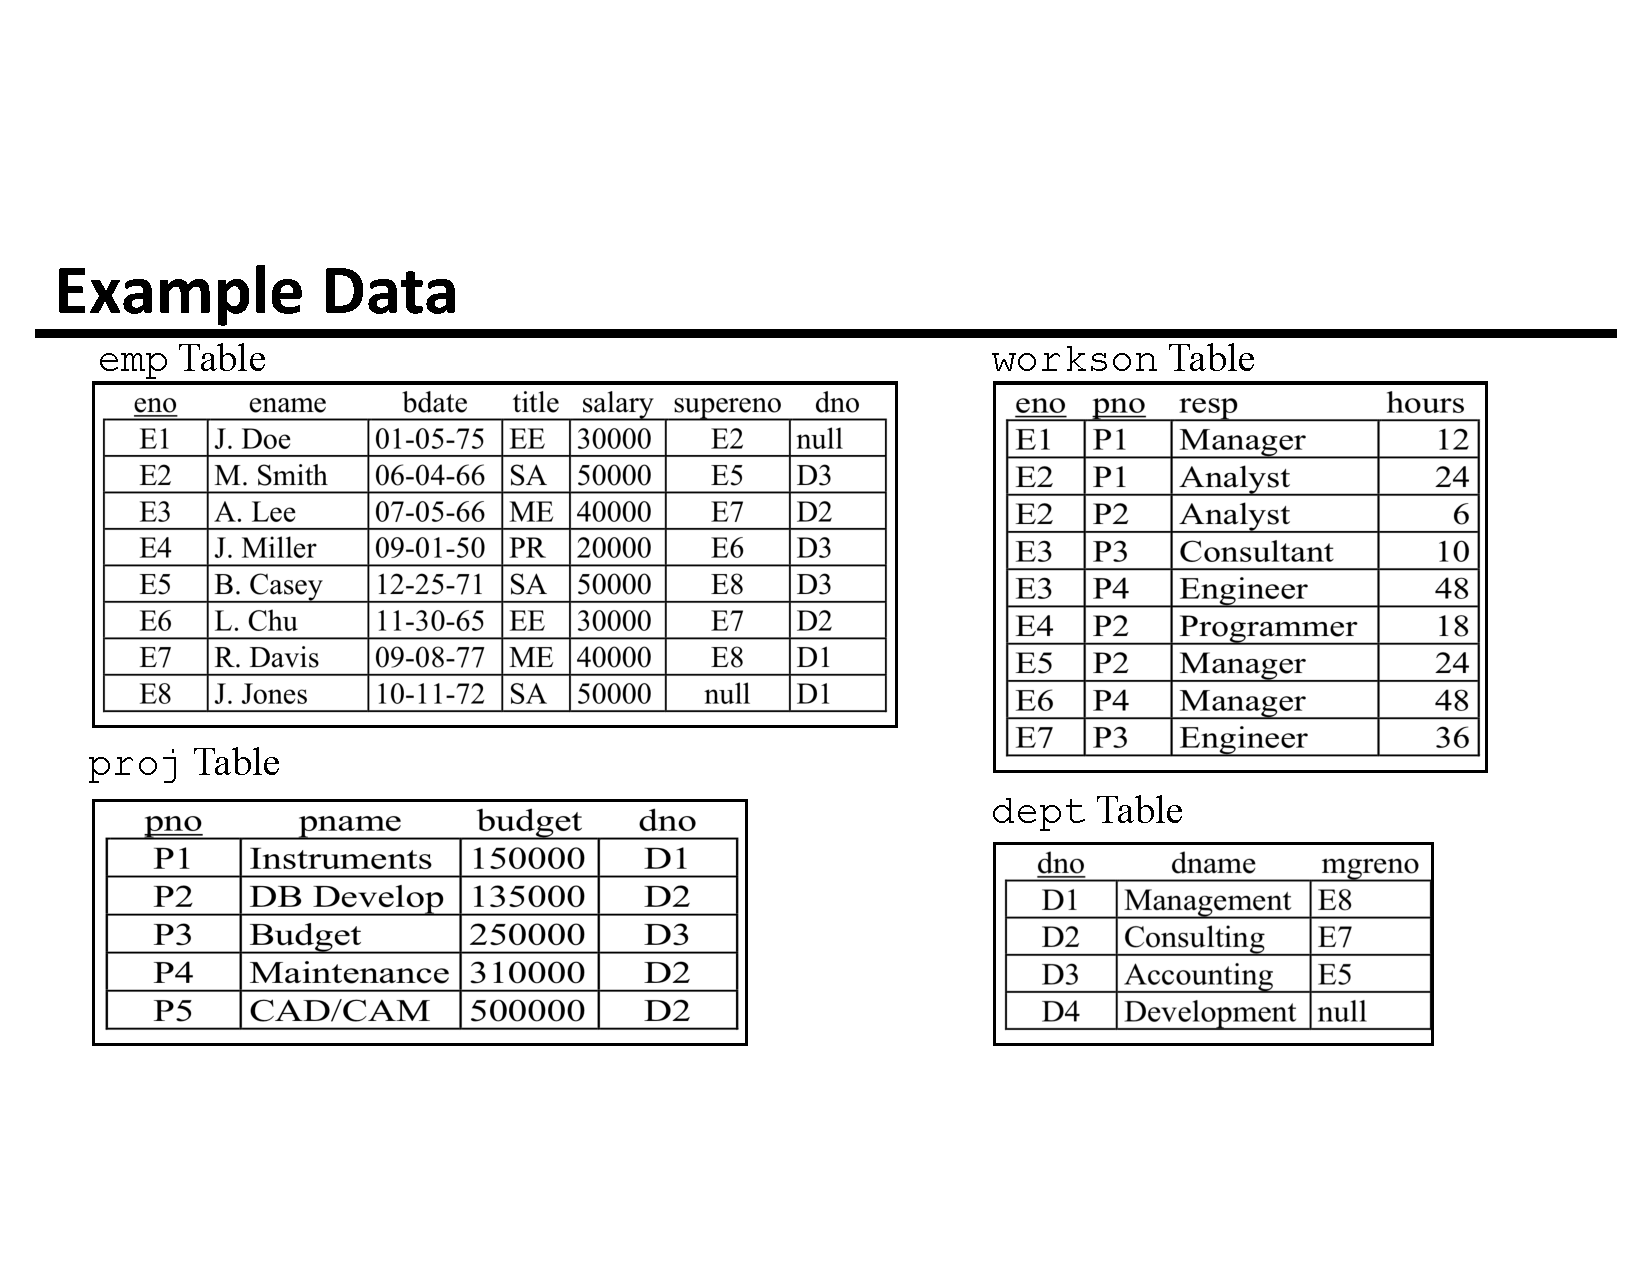
\includegraphics[width=1.17\textwidth]{ExampleData.pdf}
\end{frame}

\begin{frame}{SQL: Retrieving Only Some Columns}
The \define{projection operation} creates a new table that has some of the columns of the input table.  \nl
In SQL, provide the table in the \command{FROM} clause and the fields in the output in the \command{SELECT}.\nl
Example: Return only the {\tt eno} field from the {\tt emp} table:\\
$$ \texttt{\purple{SELECT} eno \purple{FROM} emp}$$
$$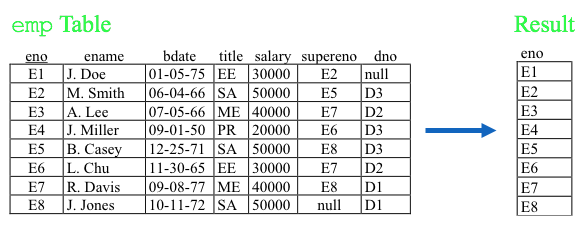
\includegraphics[width=0.9\textwidth]{SELECTFROM}$$
\end{frame}


\begin{frame}{SQL Projection Examples}
$$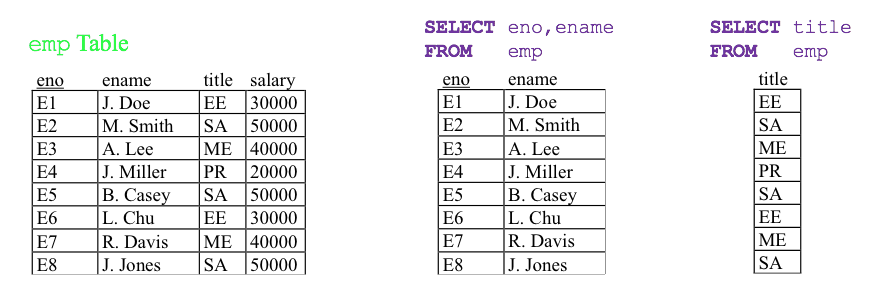
\includegraphics[width=1.\textwidth]{SQLProjection}$$
\begin{alertblock}
{Notice} 
\begin{enumerate}
\item Duplicates are not removed during SQL projection. 
\item \command{SELECT *} will return all columns. 
\end{enumerate}
\end{alertblock}
\end{frame}
%% https://softwareengineering.stackexchange.com/questions/246864/what-is-selection-and-what-is-projection
%Selecting means choosing some records from a table and leaving others out.
%
%Projecting means choosing some columns from each record and leaving others out.
%
%Broadly, the select keyword performs projection and the where keyword performs selection. (The fact that select is a language feature for choosing columns rather than rows, i.e. it performs projection, not selection, is unfortunate, but the syntax is far too established now to be corrected.)
%

\begin{frame}
To return only the distinct values from the previous example, use \command{DISTINCT}:
$$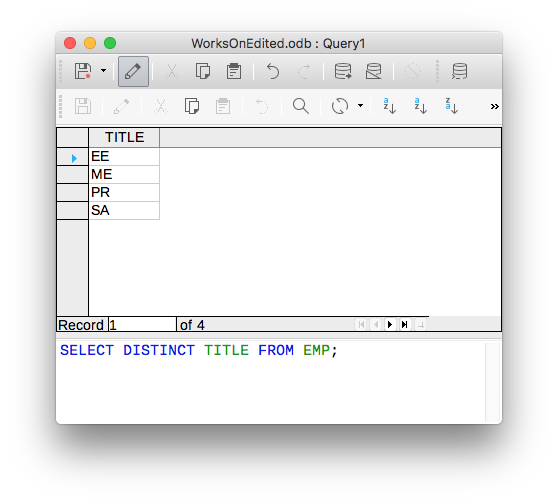
\includegraphics[width=1.\textwidth]{distinct}$$

\end{frame}



%%%%%%%%%%%%%%%%%%%%%%%%%%%%%%
\begin{frame}
\begin{columns}[T] % align columns
\begin{column}{.7\textwidth}
\begin{example}
Given this table and the following query: 
\vspace{-0.5em}
\begin{align*}
&\texttt{\purple{Select} eno, ename, salary}\\
&\texttt{\purple{From} emp }
\end{align*}
How many columns are returned?
\begin{multicols}{5}
\begin{enumerate}[A)]
\item 0 
\item 1
\item 2
\item 3
\item 4
\end{enumerate}
\end{multicols}
\end{example}
\end{column}%
\hfill%
\begin{column}{.4\textwidth}
\vspace{2em}
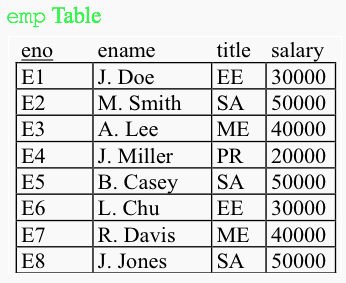
\includegraphics[width=0.95\textwidth]{img/emp.png}
\end{column}%
\end{columns}
\end{frame}


\begin{frame}<handout:0>
\begin{columns}[T] % align columns
\begin{column}{.7\textwidth}
\begin{block}{Answer}
Given this table and the following query: 
\vspace{-0.5em}
\begin{align*}
&\texttt{\purple{Select} eno, ename, salary}\\
&\texttt{\purple{From} emp }
\end{align*}
How many columns are returned?
\begin{multicols}{5}
\begin{enumerate}[A)]
\item 0 
\item 1
\item 2
\item \answer{3}
\item 4
\end{enumerate}
\end{multicols}
\end{block}
\end{column}%
\hfill%
\begin{column}{.4\textwidth}
\vspace{2em}
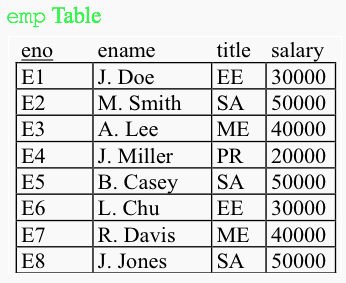
\includegraphics[width=0.95\textwidth]{img/emp.png}
\end{column}%
\end{columns}
\end{frame}


%%%%%%%%%%%%%%%%%%%%%%%%%%%%%%
\begin{frame}
\begin{columns}[T] % align columns
\begin{column}{.7\textwidth}
\begin{example}
Given this table and the following query: 
\vspace{-0.5em}
\begin{align*}
&\texttt{\purple{Select} salary}\\
&\texttt{\purple{From} emp }
\end{align*}
How many \textit{rows} are returned?
\begin{multicols}{5}
\begin{enumerate}[A)]
\item 0 
\item 1
\item 2
\item 4
\item 8
\end{enumerate}
\end{multicols}
\end{example}
\end{column}%
\hfill%
\begin{column}{.4\textwidth}
\vspace{2em}
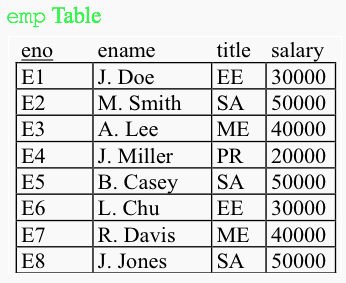
\includegraphics[width=0.95\textwidth]{img/emp.png}
\end{column}%
\end{columns}
\end{frame}


\begin{frame}<handout:0>
\begin{columns}[T] % align columns
\begin{column}{.7\textwidth}
\begin{block}{Answer}
Given this table and the following query: 
\vspace{-0.5em}
\begin{align*}
&\texttt{\purple{Select} salary}\\
&\texttt{\purple{From} emp }
\end{align*}
How many \textit{rows} are returned?
\begin{multicols}{5}
\begin{enumerate}[A)]
\item 0 
\item 1
\item 2
\item 4
\item \answer{8}
\end{enumerate}
\end{multicols}
\end{block}
\end{column}%
\hfill%
\begin{column}{.4\textwidth}
\vspace{2em}
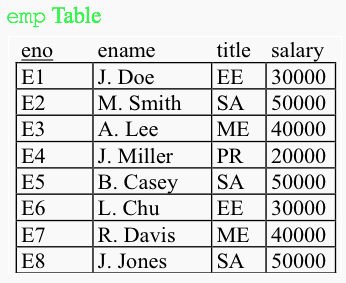
\includegraphics[width=0.95\textwidth]{img/emp.png}
\end{column}%
\end{columns}
\end{frame}









\begin{frame}{Building a \command{SELECT} SQL Query in Microsoft Access}
\begin{columns}[T] % align columns
\begin{column}{.48\textwidth}
Under {\bf Create Tab}, click on {\bf Query Design}. 
$$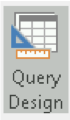
\includegraphics[width=3em]{img/QueryDesign.png}$$
Access will pop-up a window asking what table(s) you wish to query.  Select one or more.
\end{column}%
\hfill%
\begin{column}{.48\textwidth}
$$\ipic{img/MASQLquery.png}{0.8}$$
\end{column}%
\end{columns}
\end{frame}

\begin{frame}{Microsoft Access Query Interface}
\ipic{QueryInterface}{0.9}
\end{frame}


\begin{frame}{LibreOffice Query Interface}
\ipic{LibreOfficeQuery}{0.9}
\end{frame}

\begin{frame}{LibreOffice Query Interface}
\ipic{LOQuery}{0.9}
\end{frame}

\begin{frame}
\begin{itemize}
\item If you hit the Run command (
\includegraphics[width=1em]{img/runBase}\ in LibreOffice base, 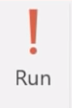
\includegraphics[width=1em]{img/runAccess}\ in Access) and results will instantly appear in a data sheet view.
\medskip
\item We can save these results in Access by clicking the "Save" icon  Toolbar.  Give your query an identifying name, eg ``Query1" for assignment question 1.
\end{itemize}
\begin{center}
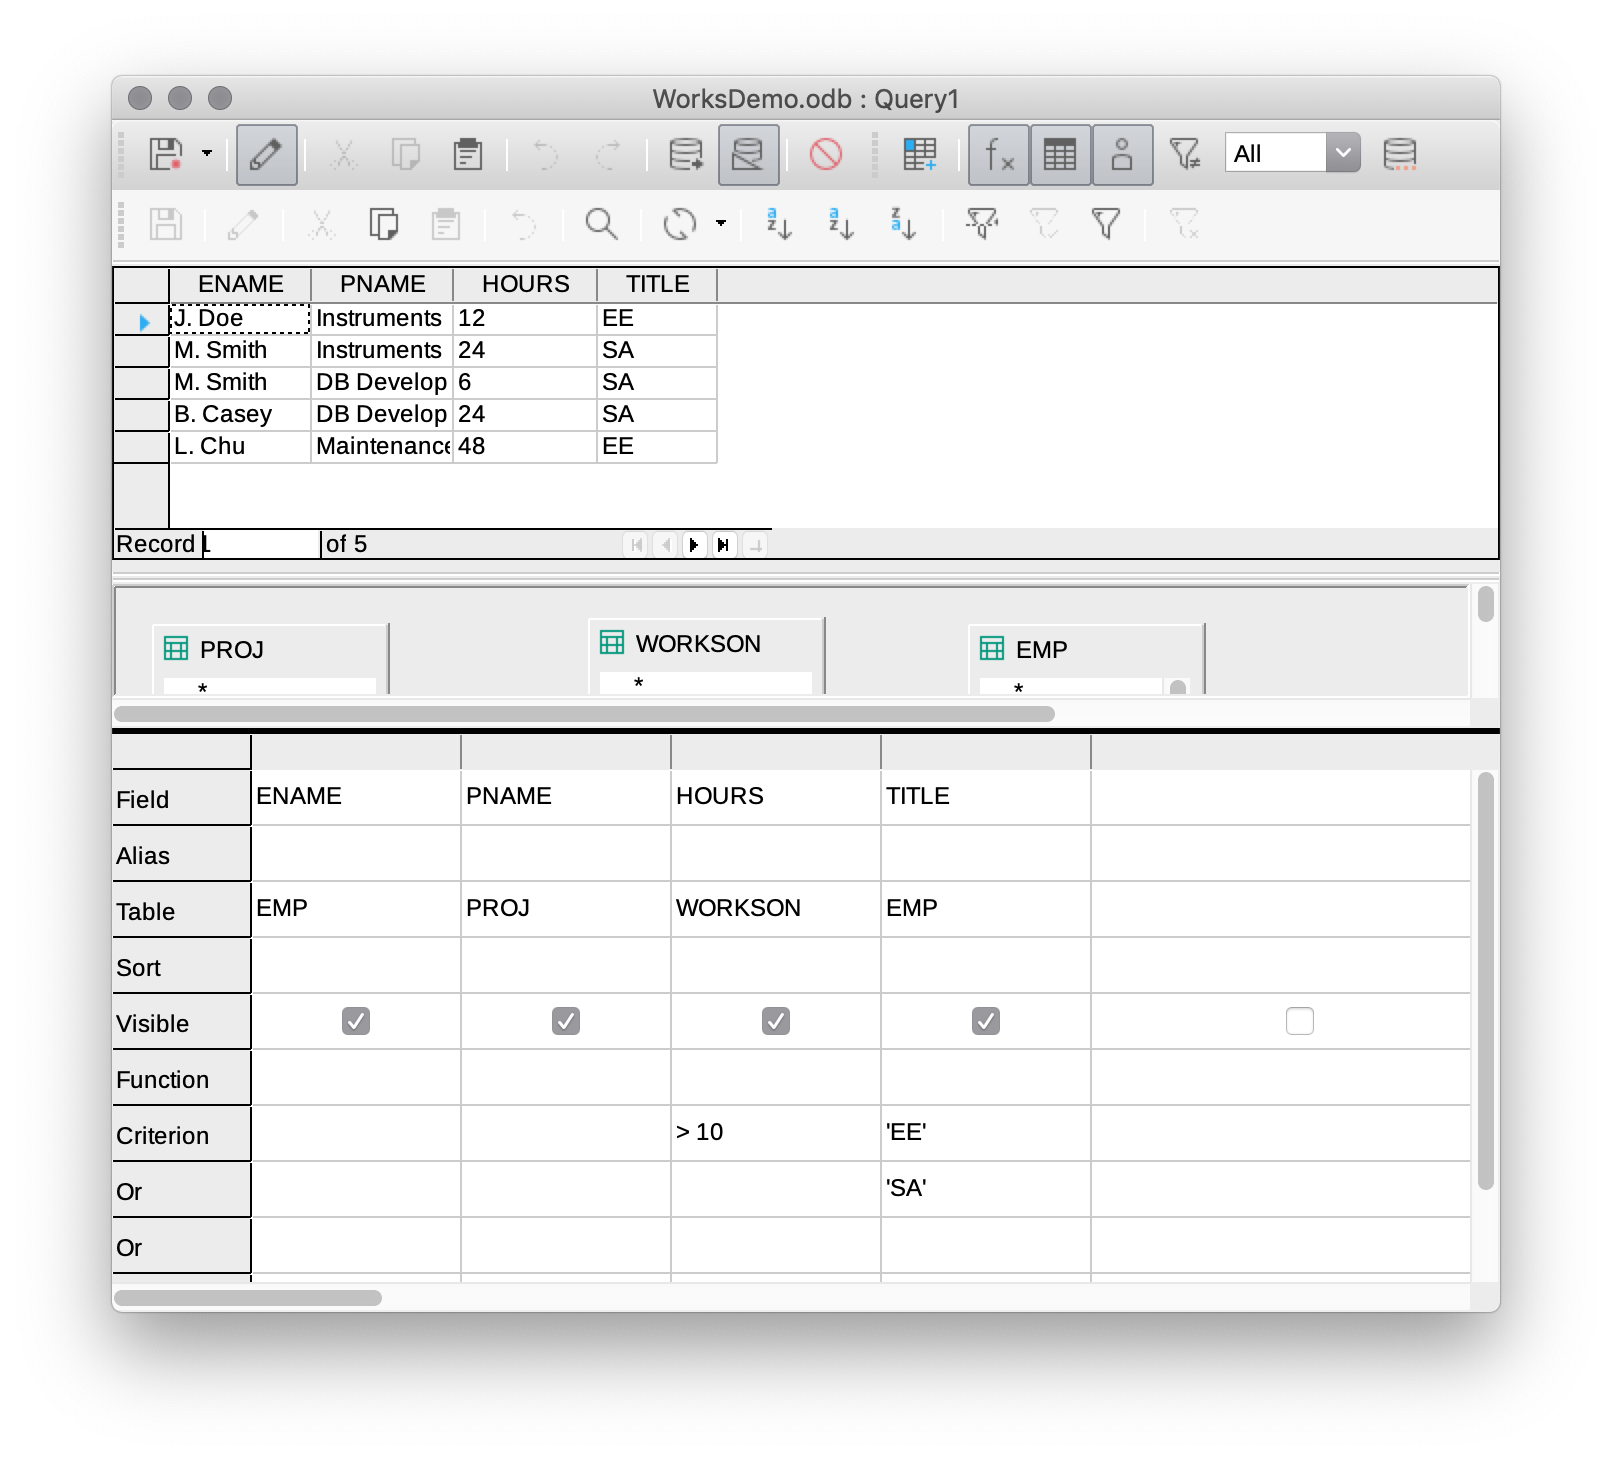
\includegraphics[width=0.6\textwidth]{img/resultsBase}
\end{center}
\end{frame}


\begin{frame}{Microsoft Access Data Sheet View}
\ipic{MOdatasheetview}{0.99}
\end{frame}

\begin{frame}{LibreOffice Preview}
To view the table: {\bf View} \ra {\bf Preview} or \keystroke{F5} or Run the Query 
\includegraphics[width=1em]{img/RunQueryButton.png}
%\ipic{LOPreview}{0.99}
\ipic{f5}{0.99}
\end{frame}


\begin{frame}{SQL Query View in LibreOffice}
The design view window in Microsoft Access and LibreOffice provide an easy way of creating SQL queries  \nl
This may be referred to as QBE or Query By Example\nl
Under the hood, these programs are creating SQL code  and runs it to give us our result set. \nl
To view that code in LibreOffice, we go to {\bf View} \ra {\bf Switch Design View On/Off}.
\begin{itemize}
\item 	`Off' will show the query in SQL
\item 	`On' will show the query graphical 
\end{itemize}
\end{frame}



\begin{frame}{LibreOffice Query Views}
$$\ipic{img/LOSQL}{0.6}$$
\begin{tikzpicture}[remember picture,overlay, xshift=0, yshift=-1em]%[xshift=65mm,yshift=-48mm,anchor=north west]
\node at (current page.center) {\includegraphics<handout:0|beamer:2>[width=.7\textwidth]{img/pretty}};
\end{tikzpicture}
Notice how the SQL code is not formatted very pretty. We can edit the white space, however, every time we close it, it will just get ugly again.
\end{frame}

\begin{frame}{Microsoft Access Queries in SQL View}
You may view your data, your query graphically, or your query in SQL.
$$\ipic{img/MAviews}{0.6}$$
For exam purposes, we will be needing to familiarize ourselves more with the SQL View. 
\end{frame}



\begin{frame}{LibreOffice base Queries in SQL View}
$$\ipic{img/sqlqbase}{0.99}$$
\end{frame}


\begin{frame}{SQL Query View in LibreOffice}
\begin{alertblock}
{Warning} Unlike the SQL statements from last lecture, the SQL view mode for queries is case sensitive. That is, it will not convert all of our lower case to upper case text as it did before (annoying I know!)
\end{alertblock}
$$\ipic{img/annoying}{0.8}$$
\end{frame}


\begin{frame}{Try it: SQL \command{SELECT} and Projection}
\begin{example}
 Using the {\tt proj} table, write these three queries:
 \begin{itemize}
\item  Show all rows and all columns.
\item Show all rows but only the {\tt pno} column.
\item Show all rows but only the {\tt pno} and {\tt budget} columns.
 \end{itemize}
%You can use Access or sqlfiddle.com.
\end{example}
\end{frame}

\begin{frame}[fragile]{Retrieving only some of the rows}
The \define{selection operation} creates a new table with some of the rows of the input table.\nl
A \emph{condition} specifies which rows are in the new table. This condition is similar to a filter in Excel. \nl
Eg. the following algorithm scans each tuple and checks if it satisfies the condition in the \command{WHERE} clause.
\begin{Verbatim}[frame=single, xleftmargin=1cm, xrightmargin=2cm, commandchars=\\\{\}]
\purple{SELECT} * \purple{FROM} proj \purple{WHERE} dno = 'D2';
\end{Verbatim}
%\vspace{-0.5em}
%\begin{align*}
%&  \texttt{\purple{SELECT} pno, pname, budget, dno} \\
%& \texttt{\purple{FROM} proj}\\
%& \texttt{\purple{WHERE} dno = `D2';}\\[-2em]
%\end{align*}
\ipic{rows}{0.9}
\end{frame}

\begin{frame}[fragile]{Selection Conditions}
\begin{itemize}
\item The condition in a selection statement specifies which rows are included.\nl

\item   It has the general form of an {\tt if} statement.\nl

\item The condition may consist of attributes, constants, comparison operators (\verb|<, >, =, !=, <=, >=|), and logical operators (\verb|AND, OR, NOT|).\nl
\item To check for {\tt NULL}s, use {\tt IS NULL}\footnote{{\tt IS NOT NULL} is used to check for non null values} which is different that checking if its equal to the empty string \verb|=''|. General syntax:
\begin{Verbatim}[frame=single, xleftmargin=0.5in, commandchars=\\\{\}]
\purple{SELECT} column_names
\purple{FROM} table_name
\purple{WHERE} column_name IS NULL;
\end{Verbatim}
\end{itemize}


\end{frame}

\begin{frame}[fragile]{SQL Selection Examples}
\begin{columns}[T] % align columns
\begin{column}{.48\textwidth}
\ipic{emp}{0.95} 

\begin{Verbatim}[xleftmargin=2em, commandchars=\\\{\}]
\purple{SELECT} *
\purple{FROM} emp
\purple{WHERE} title = 'EE'
\end{Verbatim}
%
%
%
%\vspace{-0.5em}
%\begin{align*}
%&  \texttt{\purple{SELECT} *} \\[-0.4em]
%& \texttt{\purple{FROM} emp}\\[-0.4em]
%& \texttt{\purple{WHERE} title = `EE';}\\[-2em]
%\end{align*}
\ipic{empshort}{0.95}
\end{column}%
\hfill%
\begin{column}{.48\textwidth}

\begin{Verbatim}[commandchars=\\\{\}]
\purple{SELECT} *
\purple{FROM} emp
\purple{WHERE} salary > 35000 
\purple{OR} title = 'PR'
\end{Verbatim}

%\begin{align*}
%&  \texttt{\purple{SELECT} eno, ename, title, salary} \\[-0.4em]
%& \texttt{\purple{FROM} emp}\\[-0.4em]
%& \texttt{\purple{WHERE} salary > 35000 }\\
%& \quad \texttt{\purple{OR} title = 'PR';}\\[-2em]
%\end{align*}
\ipic{emp35}{0.95}
\end{column}%
\end{columns}
\end{frame}

%%%%%%%%%%%%%%%%%%%%%%%%

\begin{frame}{Selection Question}
\begin{columns}[T] % align columns
\begin{column}{.7\textwidth}
\begin{example}
Given the {\tt emp} table and the following query, how many rows are returned?
\begin{align*}
&  \texttt{\purple{SELECT} *} \\[-0.4em]
& \texttt{\purple{FROM} emp}\\[-0.4em]
& \texttt{\purple{WHERE} title = 'SA' }\\
\end{align*}
\begin{multicols}{5}
\begin{enumerate}[A)]
\item 0 
\item 1
\item 2
\item 3
\item >3
\end{enumerate}
\end{multicols}
\end{example}
\end{column}%
\hfill%
\begin{column}{.48\textwidth}
\ipic{emp}{0.9}
\end{column}%
\end{columns}
\end{frame}


\begin{frame}<handout:0>{Selection Question}
\begin{columns}[T] % align columns
\begin{column}{.7\textwidth}
\begin{block}{Answer}
Given the {\tt emp} table and the following query, how many rows are returned?
\begin{align*}
&  \texttt{\purple{SELECT} *} \\[-0.4em]
& \texttt{\purple{FROM} emp}\\[-0.4em]
& \texttt{\purple{WHERE} title = 'SA' }\\
\end{align*}
\begin{multicols}{5}
\begin{enumerate}[A)]
\item 0 
\item 1
\item 2
\item \answer{3}
\item >3
\end{enumerate}
\end{multicols}
\end{block}
\end{column}%
\hfill%
\begin{column}{.48\textwidth}
\ipic{emp}{0.9}\\
\ipic{sol4}{0.9}
\end{column}%
\end{columns}


\end{frame}


%%%%%%%%%%%%%%%%%%%%%%%%

\begin{frame}{Selection Question2}
\begin{columns}[T] % align columns
\begin{column}{.48\textwidth}
\begin{example}
Given the {\tt emp} table and the following query, how many rows are returned?
\begin{align*}
&  \texttt{\purple{SELECT} *} \\[-0.4em]
& \texttt{\purple{FROM} emp}\\[-0.4em]
& \texttt{\purple{WHERE} salary > 40000}\\
& \quad \texttt{\purple{OR} title='PR'}
\end{align*}
\vspace{-1cm}
\begin{enumerate}[A)]
\item 0 
\item 1
\item 3
\item  4
\item $>$ 4
\end{enumerate}
\end{example}
\end{column}%
\hfill%
\begin{column}{.48\textwidth}
\ipic{emp}{0.9}
\end{column}%
\end{columns}
\end{frame}


\begin{frame}<handout:0>{Selection Question 2}
\begin{columns}[T] % align columns
\begin{column}{.48\textwidth}
\begin{block}{Answer}
Given the {\tt emp} table and the following query, how many rows are returned?
\begin{align*}
&  \texttt{\purple{SELECT} *} \\[-0.4em]
& \texttt{\purple{FROM} emp}\\[-0.4em]
& \texttt{\purple{WHERE} salary > 40000}\\
& \quad \texttt{\purple{OR} title='PR'}
\end{align*}
\vspace{-1cm}
\begin{enumerate}[A)]
\item 0 
\item 1
\item 3
\item \answer{ 4}
\item $>$ 4
\end{enumerate}
\end{block}
\end{column}%
\hfill%
\begin{column}{.48\textwidth}
\ipic{emp}{0.9}\\
\ipic{sol5}{0.9}
\end{column}%
\end{columns}
\end{frame}



%%%%%%%%%%%%%%%%%%%%%%%%

\begin{frame}{Selection Question 3}
\begin{columns}[T] % align columns
\begin{column}{.6\textwidth}
\begin{example}
Given the {\tt emp} table and the following query, how many rows are returned?
\begin{align*}
&  \texttt{\purple{SELECT} *} \\[-0.4em]
& \texttt{\purple{FROM} emp}\\[-0.4em]
& \texttt{\purple{WHERE} salary >= 40000}\\
& \quad \texttt{\purple{AND} ename > 'C'}
\end{align*}
\vspace{-1cm}
\begin{enumerate}[A)]
\item 0 
\item 1
\item 2
\item 3
\item {$\geq$ 4}
\end{enumerate}
\end{example}
\end{column}%
\hfill%
\begin{column}{.48\textwidth}
\ipic{emp}{0.9}
\end{column}%
\end{columns}
\end{frame}


\begin{frame}<handout:0>{Selection Question 3}
\begin{columns}[T] % align columns
\begin{column}{.6\textwidth}
\begin{block}{Answer}
Given the {\tt emp} table and the following query, how many rows are returned?
\begin{align*}
&  \texttt{\purple{SELECT} *} \\[-0.4em]
& \texttt{\purple{FROM} emp}\\[-0.4em]
& \texttt{\purple{WHERE} salary >= 40000}\\
& \quad \texttt{\purple{AND} ename  > 'C'}
\end{align*}
\vspace{-1cm}
\begin{enumerate}[A)]
\item 0 
\item 1
\item 2
\item \answer{3}
\item {$\geq$ 4}
\end{enumerate}
\end{block}
\end{column}%
\hfill%
\begin{column}{.48\textwidth}
\ipic{emp}{0.9}\\
\ipic{sol6}{0.9}
\end{column}%
\end{columns}
\end{frame}




\begin{frame}[fragile]{Try It: SQL \command{SELECT} and Filtering Rows}
\begin{example}
Using the {\tt proj} table, write these three queries:
\begin{itemize}
\item Return all projects with \verb|budget > $250000|.
\item Show the {\tt pno} and {\tt pname} for projects in \verb|dno = 'D1'|.
\item Show {\tt pno} and {\tt dno} for projects in \verb|dno='D1'| or \verb|dno='D2'|.
\end{itemize}
\end{example}
\end{frame}

\begin{frame}{Join Example for Combining Tables}
A \define{join} combines two tables by matching columns in each table.
\begin{columns}[T] % align columns
\begin{column}{.48\textwidth}
\vspace{-1.5em}
\begin{figure}[htbp]
\begin{center}
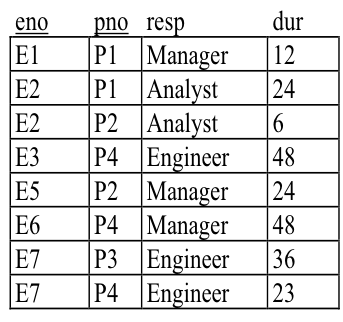
\includegraphics[width=0.9\textwidth, height=0.4\textheight]{workson}
\caption{{\tt workson}}
\end{center}
\vspace{-1.5em}
\end{figure}
\begin{figure}[htbp]
\begin{center}
\ipic{proj}{0.7}
\caption{{\tt proj}}
\label{W}
\end{center}
\end{figure}

\end{column}%
\hfill%
\begin{column}{.48\textwidth}
\begin{align*}
&  \texttt{\purple{SELECT} *} \\[-0.4em]
& \texttt{\purple{FROM} WorksOn}\\[-0.4em]
& \texttt{\purple{INNER JOIN} Proj}\\
& \quad \texttt{\purple{ON} WorksOn.pno = Proj.pno}
\end{align*}
\hspace*{-3.5em}
\ipic{innerjoin}{1.3}
\end{column}%
\end{columns}
\end{frame}



\begin{frame}[fragile]
The general syntax is:
\begin{Verbatim}[frame=single, xleftmargin=0.5in]
SELECT <columns>
FROM 
R 
<type of join> JOIN 
S
ON R.<colname>= S.<colname>;
\end{Verbatim}
Since joining tables often result in repeated field (ie. columns) we distinguish between them using {\tt table\_name.column\_name}.  \nl
N.B. the related columns will not necessarily have the same name (but oftentimes they will!)\nl

\end{frame}



\begin{frame}\ft{Joining Tables}
 When connecting tables \define R and \define S, there are four types of joins:
\begin{description}
\item [(INNER) JOIN] row in result for each row of R that matches a row of S
\item [LEFT (OUTER) JOIN] row in result for each row of R that matches a row of S OR a row of R that does not match anything in S
\item [RIGHT (OUTER) JOIN] row in result for each row of R that matches a row of S OR a row of S that does not match anything in R
\item [FULL OUTER JOIN] row in result for each row of R that matches a row of S OR a row of R that does not match anything in S OR a row of S that does not match anything in R
\end{description}
%See \href{https://www.codeproject.com/Articles/33052/Visual-Representation-of-SQL-Joins}{here} for a visual representation of joins.
\end{frame}

\begin{frame}
\href{https://www.w3schools.com/sql/sql_join.asp}{w3schools} is another good resource for learning SQL.  Here is a helpful representation of the different types of joins (where R = table1 and S=right table2).
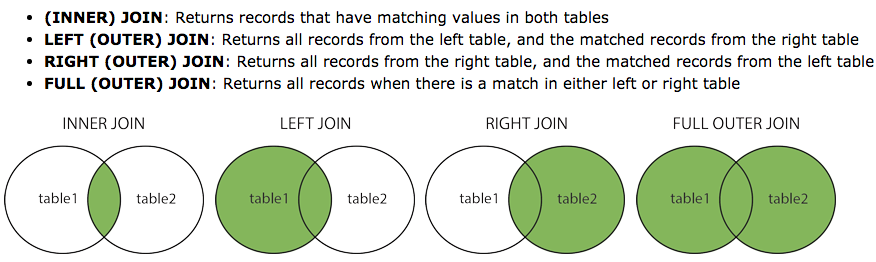
\includegraphics[width=1.\textwidth]{img/joins2}
\end{frame}




\begin{frame}
\ft{Join Example}
\command{SELECT} {\tt *} \command{FROM}  {\tt Boys}  {\tt <> } \command{JOIN}  {\tt Girls} \command{ON} {\tt Boys.Bid} = {\tt Girls.Gid};
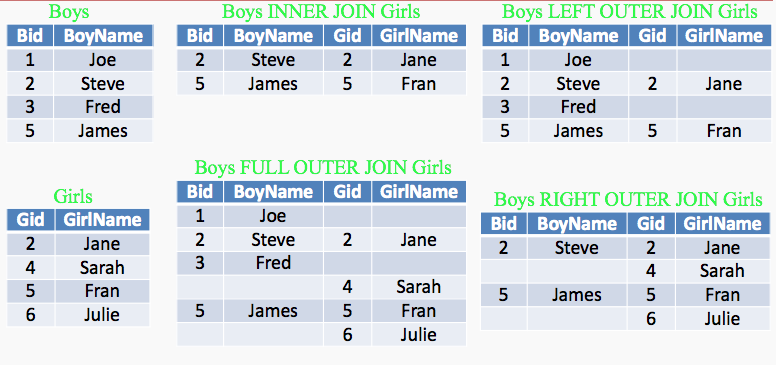
\includegraphics[width=1.\textwidth]{img/joins}
\end{frame}


\begin{frame}{Join Query with Selection Example}
You can use join, selection, and projection in the same query. Recall:
\begin{itemize}
\item \define{projection} returns \emph{columns} listed in \command{SELECT}
\item \define{selection} filters out \emph{rows} using condition in \command{WHERE}, and 
\item \define{join} combines \emph{tables} in \command{FROM} using a condition.
\end{itemize}

\begin{example}
{Return the employee names who are assigned to the 'Management' department.}
\end{example}
\end{frame}

\begin{frame}
\ipic{emp2}{0.6} \ipic{dept}{0.4}\\
\ipic{QuerySelection}{0.99}
\end{frame}

\begin{frame}{Ordering Result Data}
The query result returned is not ordered on any column by default.  We can order the data using the \orange{\tt ORDER BY} clause:
\begin{align*}
&  \texttt{\purple{SELECT} ename, salary, bdate} \\[-0.4em]
& \texttt{\purple{FROM} emp}\\[-0.4em]
& \texttt{\purple{WHERE} salary > 30000}\\
& \quad \texttt{\orange{ORDER BY} salary \green{DESC}, ename \green{ASC};}
\end{align*}
\begin{itemize}
\item \green{ASC} sorts the data in ascending order, and \green{DESC} sorts it in descending order.  The default is \green{ASC}.
\item The order of sorted attributes matters; namely, the first column specified is sorted on first, then the second column is used to break any ties, etc.
\end{itemize}
\end{frame}

\begin{frame}
In LibreOffice the order is done Left to right.  To ensure that {\tt salary} gets ordered first, add another hidden (Deselect {\bf Visible}) column with {\tt ename} to the right.
\ipic{ORDERBY}{0.9}
\end{frame}


\begin{frame}{\command{LIMIT} and \command{OFFSET}}
If you only want the first $N$ rows, use a \orange{\tt LIMIT} clause:
\begin{align*}
&  \texttt{\purple{SELECT} ename, salary \purple{FROM} emp} \\[-0.4em]
& \texttt{\purple{ORDER BY} salary \purple{DESC} \orange{LIMIT 5};}
\end{align*}
To start from a row besides the first, use \orange{\tt OFFSET}:
\begin{align*}
&  \texttt{\purple{SELECT} ename, salary \purple{FROM} emp} \\[-0.4em]
& \texttt{\purple{ORDER BY} salary \purple{DESC} \orange{LIMIT 5} \orange{OFFSET 2};}
\end{align*}
\vspace{-1em}
\begin{itemize}
\item \orange{\tt LIMIT} improves performance by reducing amount of data processed and sent by the database system.
\item \orange{\tt OFFSET 0} is first row, so \orange{\tt OFFSET 2} would return the 3rd row.
\end{itemize}
\end{frame}

\begin{frame}
\begin{itemize}
\item \orange{\tt LIMIT/OFFSET} syntax is supported differently by systems.
\item For example, Access uses 
$$\texttt{\purple{SELECT TOP 5} eno, salary \purple{FROM} emp}$$
\end{itemize}
\begin{center}
\begin{tabular}{|r|l|}
\hline
{\bf Program}  & {\bf syntax}\\
\hline
\href{https://dev.mysql.com/doc/refman/5.7/en/select.html}{MySQL}, 
\href{http://www.postgresql.org/docs/9.4/static/queries-limit.html}{PostgreSQL} 
	&  \command{LIMIT} syntax\\
\href{http://www.oracle.com/technetwork/issue-archive/2006/06-sep/o56asktom-086197.html}{Oracle} &  \command{ROWNUM} field that can be filtered in \command{WHERE}\\
\href{https://msdn.microsoft.com/en-us/library/ms189499.aspx}{SQL Server} &  \command{SELECT TOP N}\\\hline
\end{tabular}
\end{center}
(click the pink text above and \href{http://www.w3schools.com/sql/sql_top.asp
}{here} for more details.)
%References:
%MySQL- https://dev.mysql.com/doc/refman/5.7/en/select.html
%PostgreSQL - http://www.postgresql.org/docs/9.4/static/queries-limit.html
%Oracle � use ROWNUM: http://www.oracle.com/technetwork/issue-archive/2006/06-sep/o56asktom-086197.html
%SQL Server �  use TOP:https://msdn.microsoft.com/en-us/library/ms189499.aspx
%
%General: http://www.w3schools.com/sql/sql_top.asp
%

\end{frame}


\begin{frame}[fragile]{Try It: SQL \command{SELECT} with Joins and Ordering}
\begin{example}
Write these three queries:
\begin{itemize}
\item Return all projects with {\tt budget < \$500000} sorted by {\tt budget} descending.
\item List only the top 5 employees by {\tt salary} descending.  Show only their
{\tt name} and {\tt salary}. 
\item List each project {\tt pno, dno, pname}, and {\tt dname} ordered by {\tt dno } ascending then {\tt pno} ascending.  Only show projects if department name \verb|> 'D'|.  Note: This query will require a \command{join}.
\end{itemize}
\end{example}
\end{frame}

\begin{frame}
\ft{\command{SELECT} Statement Execution Order}

\begin{columns}[T] % align columns
\begin{column}{.48\textwidth}
Order written:
\begin{align*}
& {\tt \purple{SELECT} <feilds>}\\
&  {\tt \purple{FROM} <left\_table>}\\
& {\tt  \purple{JOIN} <right\_table>}\\
& {\tt \purple{ON} <join\_condition>}\\
&  {\tt \purple{WHERE} <where\_condition>}\\
&  {\tt \purple{GROUP BY} <group\_by\_list>}\\
%& = {\tt \purple{HAVING} <having\_condition>}\\
&  {\tt \purple{ORDER BY} <order\_by\_list>}
\end{align*}
\end{column}%
\hfill%


\begin{column}{.48\textwidth}
Order executed:
\vspace{1em}
\begin{enumerate}
\item FROM clause
\item JOIN clause
\item WHERE clause
\item GROUP BY clause
\item SELECT clause
\item DISTINCT clause
\item ORDER BY clause
\end{enumerate}
\end{column}%
\end{columns}
\begin{center}
Read more about it \href{https://sqlbolt.com/lesson/select_queries_order_of_execution}{here}
\end{center}
\end{frame}


\begin{frame}{Aggregate Queries and Functions}
Several queries cannot be answered using the simple form of the \command{SELECT} statement.  These queries require a summary calculation to be performed.  For example:
\begin{itemize}
\item What is the maximum employee salary?
\item What is the total number of hours worked on a project?
\item How many employees are there in department 'D1'?
\end{itemize}

To answer these queries requires the use of \define{aggregate} functions.  These functions operate on a single column of a table and return a single value.
\end{frame}

\begin{frame}{Aggregate Functions}
Five common aggregate functions are:
\begin{align*}
& \texttt{\purple{COUNT} returns the number of values in a column}\\
& \texttt{\purple{SUM} returns the sum of the values in a column}\\
& \texttt{\purple{AVG} returns the average of the values in a column}\\
& \texttt{\purple{MIN} returns the smallest value in a column}\\
& \texttt{\purple{MAX} returns the largest value in a column}
\end{align*}
Notes:
\begin{enumerate}
\item \command{COUNT, MAX}, and \command{MIN} apply to all types of fields, whereas \command{SUM} and \command{AVG} apply to only numeric fields.
\item Except for \command{COUNT(*)} all functions ignore nulls.  \command{COUNT(*)} returns the number of rows in the table.
\item Use \command{DISTINCT} to eliminate duplicates.
\end{enumerate}
\end{frame}


\begin{frame}
\ft{\command{DISTINCT} syntax}
The following selects the \textit{distinct} salaries from {\tt emp}:
\begin{itemize}
\item \texttt{\purple{SELECT DISTINCT} salary \purple{FROM} Emp}
\end{itemize}
The following counts the number of distinct salaries from {\tt emp}:
\begin{itemize}
\item \texttt{\purple{SELECT COUNT(DISTINCT }salary) \purple{FROM} Emp}
\end{itemize}
\ipic{one}{0.33}
\ipic{two}{0.33}
\ipic{three}{0.33}
\end{frame}


\begin{frame}
\ft{\command{COUNT}}
Use {\tt SELECT COUNT(*) FROM EMP;} to count all the rows including NULLS and duplicates.
\ipic{a}{0.33}
\ipic{b}{0.33}
\ipic{c}{0.33}
\end{frame}



\begin{frame}{Aggregate Function Example}
Return the number of employees and their average salary.
\begin{align*}
&  \texttt{\purple{SELECT} \purple{COUNT}(eno) AS numEmp, \purple{AVG}(salary) AS avgSalary} \\[-0.4em]
& \texttt{\purple{FROM} emp}
\end{align*}
\begin{center}
\ipic{result}{0.3}
\end{center}
Note: \command{AS} is used to rename a column in the output.\\
N.B. Aggregate functions are separated by commas just like any other field name.
\end{frame}

\begin{frame}{\command{GROUP BY} Clause}
Aggregate functions are most useful when combined with the \orange{\tt GROUP BY} clause.  \nl

The \orange{\tt GROUP BY} clause groups rows based on the values of the columns specified.\nl

When used in combination with aggregate functions, the result is a table where each row consists of unique values for the \command{GROUP BY} attributes and the result of the aggregate functions applied to the rows of that group. 
\end{frame}

\begin{frame}{\command{GROUP BY} example}
For each employee title, return the number of employees with that title.
\begin{align*}
& \texttt{\purple{SELECT} title, COUNT(eno) AS numEmp}\\
& \texttt{\purple{FROM} emp}\\
& \texttt{\purple{GROUP BY} title}
\end{align*}
$$\ipic{ex1}{0.5}$$
\end{frame}


% good grocery example : https://www.khanacademy.org/computing/computer-programming/sql/sql-basics/pt/querying-the-table
\begin{frame}{\command{GROUP BY} example}
\alert{ If a selected field is not aggregated by a function it has to be explicitily added to the GROUP BY clause!!}
\begin{align*}
& \texttt{\purple{SELECT} <A>, >B>,   aggregateFun(X) AS varName}\\
& \texttt{\purple{GROUP BY} <A>, >B>}
\end{align*}
For example. 
\begin{align*}
& \texttt{\purple{SELECT} title, COUNT(eno) AS numEmp}\\
& \texttt{\purple{FROM} emp}\\
& \texttt{\purple{GROUP BY} title} \textit{ <- without this line we get an error}
\end{align*}
$$\ipic{ex1}{0.5}$$
\end{frame}



\begin{frame}{\command{GROUP BY} example}
For each employee title, return the number of employees with that title, and the minimum, maximum, and average salary.
\begin{align*}
& \texttt{\purple{SELECT} title, COUNT(eno) AS numEmp,}\\
& \quad \texttt{\purple{MIN}(salary) AS minSal,}\\
& \quad \texttt{\purple{MAX}(salary) AS maxSal, \purple{AVG}(salary) AS avgSal}\\
& \texttt{\purple{FROM} emp}\\
& \texttt{\purple{GROUP BY} title}
\end{align*}
$$\ipic{groupby}{0.9}$$
\end{frame}

\begin{frame}{\command{GROUP BY} Facts}
\begin{enumerate}
\item You can group by multiple attributes.  To be in the same group, all attribute values must be the same.
\item Any \command{WHERE} conditions are applied before the \command{GROUP BY} and aggregate functions are calculated.
\item A column name cannot appear in the \command{SELECT} part of the query unless it is part of an aggregate function or in the list of group by attributes.
\item There is a \command{HAVING} clause that is applied \underline{after} the \command{GROUP BY} clause and aggregate functions are calculated to filter out groups. 
\end{enumerate}
\end{frame}


\begin{frame}
\ft{\command{SELECT} Statement Execution Order}

\begin{columns}[T] % align columns
\begin{column}{.48\textwidth}
Order written:
\begin{align*}
& {\tt \purple{SELECT} <feilds>}\\
&  {\tt \purple{FROM} <left\_table>}\\
& {\tt  \purple{JOIN} <right\_table>}\\
& {\tt \purple{ON} <join\_condition>}\\
&  {\tt \purple{WHERE} <where\_condition>}\\
&  {\tt \purple{GROUP BY} <group\_by\_list>}\\
&  {\tt \purple{HAVING} <having\_condition>}\\
&  {\tt \purple{ORDER BY} <order\_by\_list>}
\end{align*}
\end{column}%
\hfill%


\begin{column}{.48\textwidth}
Order executed:
\vspace{1em}
\begin{enumerate}
\item FROM clause
\item JOIN clause
\item WHERE clause
\item GROUP BY clause
\item HAVING clause
\item SELECT clause
\item DISTINCT clause
\item ORDER BY clause
\end{enumerate}
\end{column}%
\end{columns}
\begin{center}
Read more about it \href{https://sqlbolt.com/lesson/select_queries_order_of_execution}{here}
\end{center}
\end{frame}



\begin{frame}
\command{WHERE} filters \textit{before} \command{GROUP BY} whereas \command{HAVING} filters after.
\ipic{GROUPBY2}{0.33}
\ipic{WHERE}{0.33}
\ipic{HAVING}{0.33}
\end{frame}

%%%%%%%%%%%%%%%%%%%%%%%%

\begin{frame}{\command{GROUP BY} Question}
\begin{columns}[T] % align columns
\begin{column}{.48\textwidth}
\begin{example}
Given the {\tt emp} table and the following query, how many rows are returned?
\begin{align*}
&  \texttt{\purple{SELECT} title, SUM(salary)} \\[-0.4em]
& \texttt{\purple{FROM} emp}\\[-0.4em]
& \texttt{\purple{GROUP BY} title}
\end{align*}
\begin{multicols}{4}
\begin{enumerate}[A)]
\item 1 
\item 2
\item 4
\item 8
\end{enumerate}
\end{multicols}
\end{example}
\end{column}%
\hfill%
\begin{column}{.48\textwidth}
\ipic{emp}{0.9}
\end{column}%
\end{columns}
\end{frame}


\begin{frame}<handout:0>{\command{GROUP BY} Question}
\begin{columns}[T] % align columns
\begin{column}{.48\textwidth}
\begin{block}{Answer}
Given the {\tt emp} table and the following query, how many rows are returned?
\begin{align*}
&  \texttt{\purple{SELECT} title, SUM(salary)} \\[-0.4em]
& \texttt{\purple{FROM} emp}\\[-0.4em]
& \texttt{\purple{GROUP BY} title}
\end{align*}
\begin{multicols}{4}
\begin{enumerate}[A)]
\item 1 
\item 2
\item \answer{4}
\item 8
\end{enumerate}
\end{multicols}
\end{block}
\end{column}%
\hfill%
\begin{column}{.48\textwidth}
\ipic{emp}{0.9}\\
\ipic{sol10}{0.9}
\end{column}%
\end{columns}
\end{frame}


%%%%%%%%%%%%%%%%%%%%%%%%

\begin{frame}{\command{GROUP BY} Question 2}
\begin{columns}[T] % align columns
\begin{column}{.6\textwidth}
\begin{example}
Given the {\tt workson} table and the following query, how many rows are returned?
\begin{align*}
&  \texttt{\purple{SELECT} resp, pno, SUM(hours)} \\[-0.4em]
& \texttt{\purple{FROM} workson}\\[-0.4em]
& \texttt{\purple{WHERE} hours > 10 }\\[-0.4em]
& \texttt{\purple{GROUP BY} resp, pno}
\end{align*}
\begin{multicols}{5}
\begin{enumerate}[A)]
\item 9
\item 7
\item 5
\item 1
\item 0
\end{enumerate}
\end{multicols}
\end{example}
\end{column}%
\hfill%
\begin{column}{.48\textwidth}
\begin{figure}[htbp]
\begin{center}
\ipic{WORKSONQ}{0.9}
\caption{\tt workson}
\label{default}
\end{center}
\end{figure}
\end{column}%
\end{columns}
\end{frame}


\begin{frame}<handout:0>{\command{GROUP BY} Question}


\begin{columns}[T] % align columns
\begin{column}{.6\textwidth}
\begin{block}{Answer}
Given the {\tt workson} table and the following query, how many rows are returned?
\begin{align*}
&  \texttt{\purple{SELECT} resp, pno, SUM(hours)} \\[-0.4em]
& \texttt{\purple{FROM} workson}\\[-0.4em]
& \texttt{\purple{WHERE} hours > 10 }\\[-0.4em]
& \texttt{\purple{GROUP BY} resp, pno}
\end{align*}
\begin{multicols}{5}
\begin{enumerate}[A)]
\item 9
\item \answer{7}
\item 5
\item 1
\item 0
\end{enumerate}
\end{multicols}
\end{block}
\end{column}%
\hfill%
\begin{column}{.48\textwidth}
\begin{center}
\vspace{-2em}
\ipic{WORKSONQ}{0.9}\\
\ipic{sol11}{0.9}
\end{center}
\end{column}%
\end{columns}
\end{frame}



\begin{frame}{Try It: \command{GROUP BY}}
\begin{example}
Use \command{GROUP BY} and aggregation functions to answer these queries.
\vspace{-1em}
\begin{enumerate}
\item Output the total number of projects in the database.
\item Return the sum of the budgets for all projects.
\item For each department ({\tt dno}), return the department number ({\tt dno}) and the average budget of projects in that department. 
\item For each project ({\tt pno}), return the project number ({\tt pno}) and the sum of the number of hours employees have worked on that project.
\begin{itemize}
\item \alert{Challenge:} Show the project name ({\tt pname}) as well as the project number.
\end{itemize}
\item \alert{Challenge:} Show the department name ({\tt dname}), project name ({\tt pname}), and sum of hours worked on that project as well as the number of employees working on the project.
\end{enumerate}
\end{example}
\end{frame}

\begin{frame}{Putting it all together}
The steps to write an English query in SQL are:
\begin{enumerate}
\item Find the columns that you need and put in \command{SELECT} clause.
\item List the tables that have the columns in the \command{FROM} clause.  If there is more than one, join them together (using \command{JOIN}/\command{ON})
\item If you must filter rows, add a filter criteria in \command{WHERE} clause. 
\item If you need to create an aggregate, use aggregation functions (e.g. \command{COUNT}, \command{AVG}) and \command{GROUP BY}.
\item If you must filter aggregates, add a filter criteria in a \command{HAVING} clause.
\end{enumerate}
\end{frame}


\begin{frame}{Putting it all together}
Example: For each project name list the sum of the hours worked by employees working as a `Manager' on the project. 
\begin{align*}
& \texttt{\purple{SELECT} pname, \purple{SUM}(hours) as totalHours }\\
& \texttt{\purple{FROM} 	 workson \purple{INNER JOIN} proj on workson.pno=proj.pno}\\
& \texttt{\purple{WHERE}	 resp='Manager'}\\
& \texttt{\purple{GROUP BY} pname}
\end{align*}
\end{frame}


\begin{frame}{Microsoft Access Querying Summary}
\begin{enumerate}
\item Projection is performed by selecting the fields in the output in the field row in the table at the bottom of the screen.
\item  Selection is performed by entering the condition in the criteria box.  The criteria applies to the field in that column.
\item  The tables used are added to the query by the \green{Show Table}\dots option.
\item  Joins (based on relationships) are often automatically added, but if not, you can add them by selecting the join field in one table, holding the mouse button, then dragging to the join field in the other table.
\end{enumerate}


\end{frame}


\begin{frame}{Conclusion}
A \define{database} is a collection of related data.  A database system allows storing and querying a database.\nl

\define{SQL} is the standard query language for databases, although Microsoft Access also provides a graphical user interface.  \nl
\command{CREATE TABLE} creates a table.  \command{INSERT, DELETE}, and \command{UPDATE} commands modify the data stored within the database.\nl

The basic query operations are selection (subset of rows), projection (subset of columns), join (combine two or more tables), and grouping and aggregation.





\end{frame}

\begin{frame}{Objectives}
\begin{itemize}
\item Define: database, database system, schema, metadata
\item Define: relation, attribute, tuple, domain, degree, cardinality
\item SQL properties: reserved words, case-insensitive, free-format
\item Be able to create a table using CREATE TABLE command and in Microsoft Access.
\item Explain what a key is and what it is used for.
\item Use DROP TABLE to delete a table and its data.
\item Use INSERT/UPDATE/DELETE to add/update/delete rows of a table and perform same actions using Microsoft Access user interface.
\item Execute queries using SQL SELECT and using Microsoft Access user interface.
\item Sort rows using ORDER BY. Use LIMIT to keep only the first (top) N rows.
\item Use GROUP BY and aggregation functions for calculating summary data.
  \item   Given a small database write simple English queries in SQL.

\end{itemize}
\end{frame}


%\begin{frame}
%  {Questions}
%
%  \nocite{lorem,ipsum}
%  \bibliographystyle{plain}
%  \bibliography{../demo}
%
%\end{frame}

\end{document}

